\chapter{Projekt Smart Factory-Anlage}\label{ch:data}



\begin{figure}[h!]
    \centering
    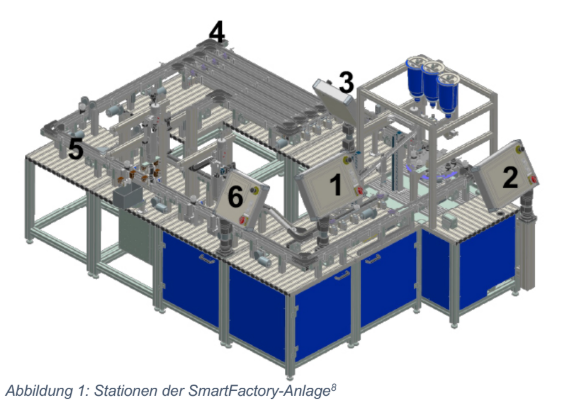
\includegraphics{figures/Screenshot 2025-01-03 124137.png}
    \caption{Stationen der SmartFactory-Anlage\cite{bee2022}} % "Abbildung 2" wird automatisch eingefügt.
    \label{Stationen der SmartFactory-Anlage} % Für spätere Verweise im Text.
\end{figure}

\section{Projekt Smart Factory-Anlage: Aufgabenstellung (evtl noch umschreiben)}\label{sec:Projekt Smart Factory-Anlage: Aufgabenstellung (evtl noch umschreiben)}

Die SmartFactory-Anlage ist eine speziell für Schulungszwecke konzipierte
Automatisierungsanlage, die von der Abteilung Expert House entwickelt wurde. Sie beinhaltet verschiedene Produkte aus dem Siemens-Produktkatalog wie zum Beispiel speicherprogrammierbare Steuerungen, Lichtsensoren und Motoren.
Meine Aufgabe bestand darin, zusammen mit 18 weiteren Studierenden die
Weiterentwicklung für diese Anlage durchzuführen. Dies umfasste sowohl die
vollständige Ausbesserung von Bugs, als auch das Testen der Robustheit der Software. Die Software wurde nach dem 
ISA-88-Standard umgesetzt und alle Erweiterungen sollen auch nach diesem hinzugefügt werden. Zur Programmierung war 
die Siemens-Automatisierungssoftware „TIA-Portal“ zur Verwendung vorgegeben. Eine weitere Anforderung war es, die 
umfassenden Dokumentationsunterlagen in Form von Word-Dokumenten für nachfolgende Studierende auszubessern und 
gegebenenfalls mit den neuen Funktionen zu erweitern. Die Nutzung des ISA-88-Standard soll gewährleisten, das die Anlage 
ohne einen Ansprechpartner aus unserem Projektteam weiterentwickelbar ist. 
(evtl auf aufteilung unit,em,cm eingehen?)


\section{Projekt Smart Factory-Anlage: Zielsetzung}\label{sec:Projekt Smart Factory-Anlage: Zielsetzung}

Das Ziel am Ende des Praxissemesters war es, die funktionsfähige
SmartFactory-Anlage Weiterzuentwickeln, ihre Robustheit zu erhöhen und dies zu präsentieren. Dafür muss für jedes 
Anlagenmodul bekannte Fehler und offene Punkte aus der LOP abgearbeitet werden, sowie bei der erkennung neuer Fehler, 
diese zur LOP hinzugefügt werden. Desweiteren müssen die Bedingungen des Projektowners, eine einheitliche HMI-Schnittstelle 
und eine leichte Bedienung der Anlage umgesetzt werden.

(Maybe auf zyklische kommunikation und buggfixes eingehen? Teil der Zielsetzung?: Bei der SmartFactory-Anlage handelt es 
sich eine Übungs- und Testanlage zu Ausbildungszwecken und dem Testen von Prototypen. Sie simuliert eine 
Flaschenabfüllungsproduktion in einem kleinen Format und soll Auszubildenden mit vielen Produkten aus dem 
Siemens-Katalog vertraut machen.
Die Anlage ist daher in sechs Anlagenmodule unterteilt, von der Materialzuführung bis hin zum abschließenden 
Recycling, jedes mit verschiedenen Schwerpunkten aber ähnlicher Hardware. Hardwaretechnisch sind alle Anlagen mit einer 
Siemens-
Simatic S7-1500 Speicherprogrammierbaren Steuerung, sowie einem Siemens-
HMI, einem Touchscreen für Statusmeldungen und Benutzereingaben und Transportbändern ausgestattet. Desweiteren sind an 
einigen Stationen pneumatisch betreibende Greifern und RFID-Schreib-Lesegeräte verbaut. Die Anlage läuft iterativ. 
Im Falle der Anlage bedeutet dies, dass am Ende des Kreislaufes, nach dem Recycling, die Flaschen, Deckel und Kugeln 
wieder für die erneute Verarbeitung bereitgestellt werden, damit sie erneut abgefüllt werden können. Die Anlage kann 
über drei Betriebsmodi, Einrichtungs-, Hand- und Automatikbetrieb und zwei Betriebsarten, Modular- und Inselbetrieb 
über das stationszugehörigen HMI gesteuert werden. Im Einrichtungsbetrieb kann der Bediener uneingeschränkt alle 
Anlagenteile bewegen, auch wenn dies zu mechanischen Fehlern führen könnte. Der Handbetrieb ermöglicht es, einzelne 
Funktionen, die sich aus der Ansteuerung mehrerer Aktoren zusammensetzen auszuführen, beispielsweise das Befüllen einer 
Flasche oder das Entleeren eines Bandes. Im Automatikbetrieb soll die Anlage vollständig automatisiert laufen und nur im 
Fehlerfall oder zum Anlegen eines Auftrags einen Bediener erfordern. Im Folgenden wird der Ablauf der verschiedenen 
Stationen der Anlage im Automatikbetrieb erläutert.)

noch teil der Zielsetzung?

Maybe als kurzbeschreibung der Anlage?

\subsection{Station 1: Modulares Produktionssystem (umschreiben)}\label{sec:Station 1: Modulares Produktionssystem}

Das Modulare Produktionssystem nimmt Flaschen und Deckel von der Recycling-Anlage entgegen und stellt diese auf Anforderung 
der Abfüllstation zur Verfügung. Sie leitet nur weiße Deckel weiter, während deckel mit einer anderen farbe aussortiert 
werden. Deckel mit unlesbaren RFID-Tag sollen grundsätzlich aussortiert werden. Sollte eine Anforderung der Abfüllstation 
erfolgen, wird die angegebene Anzahl der Flaschen gesendet und bei Anforderung ein Deckel auf die befüllte Flasche gesetzt.

\subsection{Station 2: Abfüllung (geschrieben)}\label{sec:Station 2: Abfüllung}

Die Abfüllstation hat die Aufgabe, Flaschen mit einer vorgegebenen Anzahl von Kugeln zu befüllen. Diese Anzahl wird durch 
die Erstellung von Aufträgen am HMI festgelegt. Hier kann zum Beispiel der Prozentsatz der Kugelfarbe (bei einem Maximum 
von 250 Kugeln) oder ein Absolutwert für die Anzahl der Kugeln festgelegt werden. Für das abfüllen, hat die Abfüllung drei 
Container mit jeweils, roten, blauen und gelben Kugeln. Außerdem kann die Anzahl der abzufüllenden Flaschen angegeben 
werden. Diese Anzahl wird per "On-Demand"-TCP-Verbindung an das modulare Produktionssystem gesendet. Die danach von dem 
modulare Produktionssystem gesendeten Flaschen werden durch einen Drehteller an verschiedenen Verarbeitungsstationen bewegt. 
Als erstes wird die Flasche mit des Auftrages angegebenen Anzahl an Kugeln befüllt. Dann wird ein Deckel von dem modulare 
Produktionssystem angefordert. Der Deckel wird danach mit einen drehbaren Greifer verschraubt und an der nächsten Station 
wird der Deckel mit einem RFID-Tag beschrieben. Der RFID-Tag enthält Datum und Uhrzeit der Abfüllung, sowie welcher Auftrag 
abgefüllt wurde.

\subsection{Station 3: Quality Gate (geschrieben)}\label{sec:Station 3: Quality Gate}

Das Quality Gate soll wie der Name sagt, die Auftragsdaten auf dem RFID-Tag mit dem Inhalt der Flasche abgleichen. Hierzu 
soll ein Farbsensor dienen, der die farbliche Zusammensetzung prüft. Sollte die farbliche Zusammensetzung übereinstimmen, 
wird der RFID-Tag der Flasche mit “Gut” beschrieben, sollte sie aber nicht übereinstimmen wird der RFID-Tag mit “„Ausschuss” 
beschrieben.

\subsection{Station 4: Kommissionierbahnen (geschrieben)}\label{sec:Station 4: Kommissionierbahnen}

Die Kommissionierbahnen sollen die vom Quality-Gate ankommenden Flaschen nach Auftragsnummer sortieren, hierzu wird zu 
beginn der RFID-Tag gelesen und die Flasche auf eine von vier Bahnen sortiert. Fehlerhafte Flaschen werden direkt über ein 
Ausschussband an die nächste Station weitergegeben. Sollte die Flasche “In Ordnung” sein, wird sie auf eine von vier Bändern 
sortiert. (ein auftrag pro band). Die sortierten Flaschen sollen so lange in der Station gehalten werden,
bis der entsprechende Auftrag abgeschlossen wurde oder der Bediener ein
manuelles Entleeren der Bänder anfordert.

\subsection{Station 5: Eckstation (geschrieben)}\label{sec:Station 5: Eckstation}

Das Feature der Eckstation ist, zwei Laufbänder, die wie hochklappbare Brücken fungieren. Das Hochklappen ermöglicht es, 
einen Schaltschrank in der Mitte der Anlage zu erreichen. Das Hochklappen der Laufbänder soll unterbunden werden, wenn 
noch Flaschen auf dem Laufband sind. Dies erfordert das Tracken der Flaschenanzahl und einen Stopper, um den Zulauf der 
Flaschen bei hochgeklappten Laufbändern zu verhindern und das Hochklappen bei vollem Laufband zu verhindern. Ist das 
Laufband voll, wird der Zulauf durch den Stopper verhindert.

\subsection{Station 6: Recycling (geschrieben)}\label{sec:Station 6: Recycling}

Die Recyclingstation recycelt alle ankommenden Flaschen, also alle aus erfolgreich erfüllten Aufträgen und alle aussortierten
Flaschen. Der Flaschendeckel wird mit einem Greifer entfernt und auf ein anderes Laufband gesetzt. Danach wird die Flasche 
angehoben und die Kugeln über einem Trichter entfernt. Die Kugeln werden daraufhin mit einem Farbsortierer und Luftdruck in 
die farblich übereinstimmenden Container an der Abfüllung geschossen, und die Flasche wird auf das Laufband zum modularen 
Produktionssystem gesetzt.

\subsection{Netzwerkverbund (geschrieben)}\label{sec:Netzwerkverbund}

Alle Anlagenteile sind mit Ethernet mit dem Einschaltschrank verbunden und bilden damit ein Subnetz. Dies ermöglicht eine 
effiziente und stabile Kommunikation zwischen den verschiedenen Stationen der Anlage und ermöglicht das senden und empfangen 
von Daten.
Die gesamte Kommunikation der Anlage erfolgt “On-Demand” und passiert dadurch nur wenn sie von einer anderen Station 
angefordert wird. Dies minimiert unnötigen datenverkehr und trägt dadurch zur Reduzierung der verbrauchten Ressourcen bei.

\section{Projekt SmartFactory-Anlage: Projektorganisation (geschrieben)}\label{sec:Projekt SmartFactory-Anlage: Projektorganisation (am ändern)}

Das Projektteam besteht aus ... Informatikstudenten und ... Elektro- und Informationstechnikstudenten sowie drei 
Fachbetreuern. Diese haben uns als "Product Owner" im Projekt unterstützt und geleitet.  

Das gesamte Projekt wurde auf Scrum basierend durchgeführt. Allerdings wurde, wie in Abschnitt 1, "Einleitung", erläutert, 
sowohl bei uns, den Informatikern, als auch bei den Elektro- und Informationstechnikern, die Phase im Expert House durch die 
SPE-Phase unterbrochen, dies allerdings zu unterschiedlichen Zeitpunkten. Dadurch wurde in den ersten acht Wochen von allen 
gemeinsam am Projekt gearbeitet, in den folgenden acht Wochen nur von den Elektro- und Informationstechnikern, und in den 
letzten acht Wochen ausschließlich von uns Informatikern.  

Dies führte dazu, dass an den Übergabepunkten große und kleine Änderungen klar an die "Nachfolger" übergeben werden mussten.
Gleichzeitig war es essenziell, die Dokumentation stets auf dem aktuellen Stand zu halten, um eine reibungslose Weiterarbeit 
zu ermöglichen.  

Dies passte gut, da wir unser Team mit Scrum organisiert haben. Dadurch stimmten wir uns gemeinsam, Betreuer und 
Auszubildende, in Daily-Meetings ab. Wir arbeiteten in Zwei-Wochen-Sprints, die jeweils mit einer Vorstellung der 
Ergebnisse an die Stakeholder endeten. Eine zentrale Rolle spielte die "List of Open Points" (LOP), die zur Dokumentation 
von bestehenden Fehlern und Mängeln genutzt wurde.  

Die LOP war in Dringlichkeitsstufen unterteilt:
\begin{itemize}
    \item \textbf{Sehr wichtig:} Prozessbeendende Fehler oder solche, die mechanische Schäden verursachen könnten.
    \item \textbf{Mittel:} Fehler, die den Prozess nicht vollständig stoppen, aber zu Fehlern in der Verarbeitung von Flaschen führen.
    \item \textbf{Niedrig:} Fehler mit geringeren Auswirkungen, z. B. das Herausfallen einer Kugel bei der Initialisierung der Abfüllstation.
\end{itemize}


Die Stakeholder legten diese Prioritäten fest. Für jeden Sprint suchten sich die Verantwortlichen der jeweiligen Station 
die wichtigsten Aufgaben mit der höchsten Priorität heraus und arbeiteten diese ab.  

Gerade zu bearbeitende Aufgaben und bereits abgeschlossene wurden in ein Kanban-Board eingetragen. Dies half, den Fortschritt 
zu visualisieren und machte in den Daily-Meetings deutlich, welche Aufgaben eventuell vom Plan abwichen. Dadurch konnten 
notwendige Anpassungen schnell besprochen und vorgenommen werden, um weiterhin das Projektziel in der gegebenen Zeit zu 
erreichen.  

Obwohl wir uns nicht strikt an Scrum hielten, ergab dieser Ansatz aus unserer Sicht Sinn. Der Überblick über die aktuellen 
Aufgaben war so deutlich besser, und die Verständlichkeit in den Meetings wurde durch die Visualisierung wesentlich 
erleichtert.

Das Kanban-Board wurde in folgende Bereiche unterteilt:
\begin{itemize}
    \item \textbf{Aufgaben:} Hier befinden sich alle Aufgaben, die im aktuellen Sprint erledigt werden müssten, mit denen 
    sich aber noch niemand befasst hat.
    \item \textbf{In Bearbeitung:} Hier wurden die aktuell bearbeiteten Aufgaben gesammelt.
    \item \textbf{Internes Review:} Wurde eine Aufgabe abgeschlossen, wurde das Ergebnis zunächst durch einen weiteren 
    Studierenden überprüft.
    \item \textbf{Ready for Review:} Eine von einem Studierenden als in Ordnung befundene Aufgabe wird noch ein weiteres 
    Mal durch einen Betreuer geprüft.
    \item \textbf{Nacharbeiten:} Wurde eine durchgeführte Aufgabe entweder von einem Betreuer oder einem Studierenden als 
    nicht in Ordnung befunden, oder es traten im Projektverlauf Probleme damit auf, ist sie in diesem Bereich zu finden.
    \item \textbf{Erledigt:} In diesem Bereich befinden sich schließlich komplett abgeschlossene Aufgaben.
\end{itemize}

Des Weiteren haben wir mit dem Siemens-Multiuser-Server gearbeitet, eine  speziell angepasste Lösung für die Zusammenarbeit an 
Automatisierungsprojekten. Das bedeutet, dass jeder Studierende eine lokale 
Instanz des Projekts hatte, diese bearbeiten und an der Anlage testen konnte. Große Änderungen konnten dann auf einen 
GIT-ähnlichen Server hochgeladen werden, von dem alle anderen Instanzen diese Änderungen wieder herunterladen konnten. 
Außerdem konnte man über ein File-Locking-System bei Dateien, an denen man gerade arbeitete, festlegen, ob ein Konflikt 
besteht, wenn zwei Studierende gleichzeitig an derselben Datei arbeiten. Dies hat "Merge-Konflikte" und den Verlust 
von Code verhindert, die Zusammenarbeit erleichtert und ermöglicht eine grundlegende Versionskontrolle.

\section{Projekt SmartFactory-Anlage: Projektverlauf (umschreiben)}

\textbf{"Begriffsklärung „TIA Portal“:}

Im nachfolgenden Abschnitt wird das TIA-Portal mehrfach thematisiert. Dabei handelt es sich um die 
Entwicklungsumgebung für alle Automatisierungsprodukte von Siemens \cite{bee2022}.

Die Prozesslogik für SPS (Speicherprogrammierbare Steuerungen) lässt sich in verschiedenen Programmiersprachen umsetzen, 
darunter FUP (Funktionsplan), AWL (Anweisungsliste) und SCL (Structured Control Language). Für die SmartFactory-Anlage 
wurde festgelegt, die Programmierung bedarfsgerecht in FUP und SCL durchzuführen.

Da eine PLC (Programmable Logic Controller) als Echtzeitsystem zyklisch arbeitet, sie führt 
Berechnungen durch und aktualisiert Ausgaben in festen Intervallen, sind bei der Programmierung spezielle Anforderungen 
zu beachten. Um diesen Anforderungen gerecht zu werden, stehen verschiedene Konzepte zur Verfügung:

\begin{itemize}
    \item \textbf{Funktion:} Ähnlich wie eine Methode in C\#, ermöglicht eine Funktion die Verarbeitung von Übergabeparametern 
    und die Berechnung entsprechender Ausgabewerte. Allerdings sind diese Ausgabewerte nicht persistent, da sie in jedem 
    Programmzyklus neu berechnet werden.
    \item \textbf{Funktionsbaustein:} Ein Funktionsbaustein bietet dieselben Möglichkeiten wie eine Funktion, jedoch mit der 
    zusätzlichen Fähigkeit, Daten über mehrere Zyklen hinweg zu speichern.
    \item \textbf{Datenbaustein:} Ein Datenbaustein dient der persistenten Speicherung von für das Programm relevanten Daten. 
    Wird ein Funktionsbaustein erstellt, wird automatisch ein zugehöriger Datenbaustein zur Speicherung seiner Daten angelegt.
    \item \textbf{User Defined Datatype (UDT):} Ein UDT ist ein benutzerdefinierter Datentyp, der individuell vom 
    Programmierer erstellt werden kann.
\end{itemize}

\textbf{Auftaktwoche:}

Noch vor dem offiziellen Start des Projekts wurde in meiner Abteilung eine Auftaktwoche organisiert, die dazu diente, 
uns auf die bevorstehenden Aufgaben vorzubereiten. Der Schwerpunkt lag darauf, unser Wissen und unseren Umgang mit dem 
TIA Portal aufzufrischen. Obwohl wir als dual Studierende bereits einen zweiwöchigen Kurs zur Nutzung der Software 
absolviert hatten, fehlte uns durch ein Semester ohne praktische Anwendung die nötige Routine. In dieser Woche bestand 
unsere Aufgabe darin, die Steuerung eines Aufzugs mit fünf Stockwerken zu programmieren. Dabei wurden uns auch 
Programmierkonzepte wie die „State Machine“ vermittelt, die später eine wichtige Rolle bei der Entwicklung der 
SmartFactory-Anlage spielten.

\textbf{Hands-On SmartFactory-Anlage:}

Nach der Auftaktwoche wurden wir zufällig in Teams von zwei bis drei Personen eingeteilt, um die SmartFactory-Anlage 
in Betrieb zu nehmen. Ziel war es, am Ende der Woche eine Flasche, mit dem bereits bestehenden Code, vollständig durch 
die Anlage zu führen. Jedem Team wurde dabei eine spezifische Station zugewiesen. Ich war für die Abfüllstation zuständig. 
Die Aufgabenstellung war bewusst vage gehalten, um uns die Möglichkeit zu geben, die Anlage eigenständig kennenzulernen. 
Das Ergebnis bei der Abfüllstation bestand darin, das angefragte Flaschen und Deckel richtig für erstellte Aufträge 
verwendet wurden und ein Betriebsbeendender des ersten Laufbandes behoben wurden. Allerdings wurden auch einige neue Punkte, 
wie die fehlerhafte Kalibrierung des Drehtellers oder die fehlende Initalisierungsfahrt, in die LOP (List of Open Points) 
nachgetragen. Nach Abschluss dieser Aufgabe führten wir ein „Lessons Learned“ durch. Die wichtigste Erkenntnis hierbei war, 
dass die Anlage ohne einen sorgfältig erarbeiteten Plan und ein durchdachtes Konzept nicht effektiv in Betrieb 
genommen werden kann.

\textbf{Konzeptionierung nach ISA-88:}

Die Software der Anlage wurde gemäß dem ISA-88-Standard konzipiert. Dieser Standard legt fest, dass die Software in 
wiederverwendbare Module für Bauteile und Baugruppen strukturiert wird. Die Module wurden in die folgenden Typen unterteilt:

\sloppy
\begin{itemize}
    \item \textbf{Control Modul:} Ein Control Modul repräsentiert einzelne Bauteile, die an jeder Station der Anlage
    vorkommen. Ein typisches Beispiel ist ein Sensor. Obwohl an der Anlage verschiedene Sensortypen verbaut sind, teilen 
    sie alle die grundlegende Funktion, ein Bit umzuschalten. Das Control Modul \texttt{CM\_BinarySensor} soll so entwickelt 
    werden, dass es universell für alle Sensortypen einsetzbar ist, wobei lediglich die Hardwareadresse des jeweiligen 
    Sensors angegeben werden muss.

    \item \textbf{Equipment Modul:} Equipment Module bestehen aus einer Kombination mehrerer Control Module und bilden 
    komplexere Baugruppen ab. Beispielsweise sind an den Förderbändern der SmartFactory-Anlage neben Sensoren auch 
    Pneumatikzylinder verbaut. Da die Anzahl der Control Module pro Förderband variieren kann, wurde das Equipment Modul 
    \texttt{EM\_Conveyor} so gestaltet, dass es eine beliebige Anzahl an Control Modulen unterstützt und flexibel 
    konfigurierbar ist.

    \item \textbf{Unit:} Die Unit bildet die spezifische Prozesslogik eines Anlagenmoduls ab und implementiert die 
    erforderlichen Programmabläufe.
\end{itemize}

Die Struktur eines nach ISA-88 entworfenen Systems ist hierarchisch organisiert. In diesem Aufbau kommuniziert eine Unit 
ausschließlich mit Equipment Modulen, während Equipment Module sowohl mit Units als auch mit Control Modulen interagieren. 
Control Module hingegen stehen nur in Verbindung mit Equipment Modulen.

\begin{figure}[h!]
    \centering
    \includegraphics*{figures/Screenshot 2025-01-03 201917.png}
    \caption{ISA-88 Modulhierarchie\cite{bee2022}} % "Abbildung 2" wird automatisch eingefügt.
    \label{fig:isa88-modulhierarchie} % Für spätere Verweise im Text.
\end{figure}

\textbf{Bibliotheksverantwortlicher (erweiternder Aufgabenbereich):} 

Mir wurde ein erweiterter Aufgabenbereich in Form des Bibliotheksverantwortlichen zugewiesen. Meine Aufgabe bestand darin, 
die Projektbibliothek des Multiuser-Servers konsistent zu halten. Dies ist notwendig, da Programmbausteine gemäß dem 
ISA-88-Standard, wie beispielsweise \textit{Control Modules} oder \textit{Equipment Modules}, von mehreren Instanzen im 
Projekt genutzt werden können.

Ein Lichtsensor kann beispielsweise Teil eines Förderbands oder eines Drehtellers sein. Um doppelten Code zu vermeiden und 
die Erweiterbarkeit so hoch wie möglich zu halten, wird im Code, wenn ein Lichtsensor benötigt wird, der Baustein aus der 
Projektbibliothek verwendet. Dieser Baustein wird im Projekt als neue Instanz des Bausteins aus der Projektbibliothek 
eingefügt. Möchte man den genannten Lichtsensor aktualisieren, werden alle Instanzen im Projekt sowie in der 
Projektbibliothek aktualisiert.

Da die Projektbibliothek versionsabhängig arbeitet, kann es vorkommen, dass jemand am Förderband eine Änderung vornimmt, die 
nicht mit der neuen Version des Lichtsensors kompatibel ist. Dies würde zu einem Ausfall der Lichtsensoren am Förderband 
führen. Ebenso könnte es passieren, dass auf dem Förderband noch eine ältere Version des Lichtsensors ohne die aktuellen 
Änderungen verwendet wird. Dies führt zu Inkonsistenzen, die von mir bereinigt werden mussten.

\textbf{flaschenmanagment in der unit:} 
wie es war -> wie es werden soll (z.b. auftrag abarbeiten wenn keine weitere flasche kommt oder ersten drei flaschen für neuen auftrag verwendet)
leerfahren in der unit (bei unbekannten Flaschen)
current order abbrechen 

\textbf{Drehteller:} 
fehlerfindung der knöpe -> Initalisierungsfahrt 

\textbf{Trusted Tracebility:} 
rfid überschreibung abgepasst + anzeige auf dem bildschirm 

\textbf{Kommunikation:} 
zyklisch und unitlogik zwischen mps und Abfüllung 
zwischen abfüllung und quality gate 

%/////////////////////////////////////////////////////////////////////////////////////////////////////
\section{Projekt SmartFactory-Anlage: Ergebnis (umschreiben)}

Das Endergebnis des Projekts ist zum Zeitpunkt der Erststellung dieses Berichts
noch nicht vollständig vorhersehbar. Allerdings wurden bereits wichtige
Meilensteine zur Erreichung des Ziels nach Vorgabe erreicht. Mit Ausnahme des
Betriebsmodi und Error-Handlings wurden alle Equipment- und Controlmodule
fertig implementiert. Die Eckstation sowie die Kommissionierbahnen weisen
bereits einen funktionsfähigen Automatikbetrieb nach Pflichtenheft auf. Basierend
auf den Rückmeldungen der Projektmitglieder in den täglichen Meetings lässt sich
prognostizieren, dass innerhalb der kommenden Woche auch die Recyclingstation
und das Quality-Gate diesen Status erreichen werden. Der Projektfortschritt folgt
aktuell noch dem Zeitplan und ein Projekterfolg ist deshalb absehbar. Sollte
allerdings der Fall eintreten, dass der Projektfortschritt zum Ende des
Praxissemesters nicht vollständig der Zielsetzung entspricht, ermöglichen die
sorgfältig ausgearbeiteten Konzeptdokumente eine erfolgreiche Projektadaption
durch zukünftige Studierende.

